

\label{sub:SpecO}


Our assertion language %\AssertLang, 
{supports} standard  as well \emph{object-capability} assertions. 
 The  standard assertions  include the values of fields, implication, quantification etc, as well as ghost fields; the latter can represent user-defined predicates. 
The  object capability assertions express restrictions of an object's eventual authority on some other object.
%{They are about objects being
%\emph{external} or about   \emph{protection} -- inspired by the OCAP literature.}
%$\footnoteSD{TODO say how these relate with capability lit;  compare
%with OOPSLA.}
%KJX DIDTHIS IN relateld work, WHERE IT BELONGS
%
%We define the meaning of  standard'' assertions in section \ref{sect:semantics:assert:standard}, 
%and the meaning of the   object-capability assertions in  sections \ref{sect:semantics:assert:prtFrom}
%and  \ref{sect:semantics:assert:prt}.


%\subsection{Syntax of \AssertLang}
%The syntax of \AssertLang  is given in Definition \ref{f:chainmail-syntax}.
%Standard assertions may be  extended expressions,   queries on an object's class, or the usual connectives and quantifiers. 
%{Extended expressions, $\re$, may include addresses -- the reason is discussed later.}

%\susan{why extended expression rather than just expression?}

\begin{definition}
\label{def:assert:syntax}
Expressions, $\re$, and assertions, $A$,  are defined as follows:

\label{f:chainmail-syntax}
$
\begin{syntax}
\syntaxElement{\re}{}
		{
		\syntaxline
				{\prg{true}}
                                {{\alpha}}
				{{x}}
                                {\re.f}
				{\re.f({\overline{\re}})}
		\endsyntaxline
		}
\endSyntaxElement

\syntaxElement{A}{}
		{
		\syntaxline
				{{\re}}
				{{\re} : C}
				{\neg A}
				{A\ \wedge\ A}
				{\all{x:C}{A}}
				{\external{{\re}}}
 				{\protectedFrom{{\re}} {{\re}}} 
				 {\inside {{\re}}} 
		\endsyntaxline
		}
\endSyntaxElement\\
\end{syntax}
$
%In the above, we expect that
\footnote{Assertions  may contain addresses; \eg   $\alpha.bal > 700$. While addresses make little sense in user-written assertions, they are useful when giving semantics to universal quantifiers 
\cf Def. \ref{def:chainmail-semantics}.(\ref{quant1}), {when the local map changes \eg upon call and return, and in general,} for two-state invariants, \cf Def. \ref{def:necessity-semantics}}

\vspace{.1cm}

{$\fv(A)$ returns the free variables in $A$; for example, $\fv(a\!:\!Account \wedge \forall b:int.[a.\balance = b])$=$\{ a \}$.} 
% {{Moreover, $\fv(A)$ is defined in the obvious way to to return   the free variables in $A$; for example, $\fv(a\!:\!Account \wedge \forall b:int.[a.\balance = b])$=$\{ a \}$.}}
Here 
$f$ stands  for a field, or a ghost  field, but not a method -- \ie no
side-effects.\footnote{The syntax does  not distinguish between fields and ghost fields.
For instance, $\prg{a}.\prg{\balance}$ may, in some modules (\eg in \ModA), be a field lookup, while in others (e.g. when the balance is defined though an entry in a lookup table) may involve executing a ghost function. 
}
\end{definition}

\forget{
\noindent
\textbf{NOTES}  \notesep % Extended expressions, $\re$, and therefore also 
 Assertions  may contain addresses; \eg   $\alpha.bal > 700$. 
{While addresses make little sense in user-written assertions, they are useful when giving semantics to universal quantifiers 
\cf Def. \ref{def:chainmail-semantics}.(\ref{quant1}), {when the local map changes \eg upon call and return, and in general,} for two-state invariants, \cf Def. \ref{def:necessity-semantics}.(2).}
\notesep The syntax does  not distinguish between fields and ghost fields. For instance, $\prg{a}.\prg{\balance}$ may, in some modules (\eg in \ModA), be a field lookup, while in others (e.g. when the balance is defined though an entry in a lookup table) may involve executing a ghost function. 
% -  $\external {\re}$ is short for $\neg \internal {\re}$. We use these forms freely in the subsequent text without further definition.
%\kjx{These NOTES seem to make heavy work of mostly trivial points
%{{SD: WIll work on that}}
% \footnoteSD{{\textbf{NOTE for us} It also allows assertions like $a1.passwd \neq a2.passwd$, whereas in the past we would have written as $\exists x,y.[\ a1.passwd=x \wedge  a2.passwd=y \wedge x\neq y\ ]$.}} \footnoteSD{{TODO compare with oopsla }}
}


\begin{definition}[Shorthands] 
{We write $\internal{\re}$ for $\neg (\external {\re})$}, and
$\extThis$. resp. {$\intThis$} for $\external{\prg{this}}$ resp. $\internal{\prg{this}}$. %, and $\re:\prg{intl}$ as short for $ \neg \external {\re}}$. 
Forms as $A \rightarrow A'$,  $A \vee A'$, and $\exists x:C.A$  can be encoded.
%; we use these forms freely in the subsequent text.
% without further definition.
\end{definition}



\begin{definition}[Satisfaction  of Assertions by module and  state] 
\label{def:chainmail-semantics-all}
\label{def:chainmail-semantics}
is expressed through  through \ \ $\satisfiesA{M}{\sigma}{{A}}$ \ \ \ and defined by cases on the shape of $A$, in definitions \ref{def:chainmail-semantics}, \ref{def:chainmail-protection-from}, and 
 \ref{def:chainmail-protection}.
\end{definition}

\footnoteSD{say why we split the def into three defs.} 
\noindent
\textbf{NOTE}  While execution takes place in the context of one or more modules, $\Mtwo$, satisfaction of assertions considers \emph{exactly one} module  $M$ -- the internal module. 
%{This is not surprising since the goal of this work is to ensure that external modules cannot break our (internal) module's assertions.}
%\footnoteSD{We need to have clarified internal module earlier.} 
%In most cases, satisfaction depends only on the state $\sigma$, but 
% in some cases it also depends on the module $M$: namely execution of extended expressions   
{$M$} is used % might need to 
 to look up the definitions of ghost fields, and to find class definitions to determine whether an object is  external.
% -- c.f. Def. \ref{def:chainmail-semantics}, cases (\ref{cExpr}),  (\ref{cInternal}). %,  and (\ref{cExternal}) .

\subsection{Semantics of assertions % \AssertLang 
-- first part}
\label{sect:semantics:assert:standard}

% An illustration of the concept of reachable appears in the next subsection, in Fig. \ref{fig:Relevant}.
To determine satisfaction of an expression, we    use the evaluation relation, $\eval{M}{\sigma}{e}{v}$,
which says that the expression $e$ evaluates
to value $v$ in the context of state $\sigma$ and module $M$.
As expressions in \LangOO may be recursively defined, their evaluation 
need not   % may not necessarily 
 terminate. Nevertheless, the logic of $A$ remains classical because recursion is restricted
to expressions, and not generally to assertions.
\footnoteSD{
The semantics of $\hookrightarrow$ {is} unsurprising 
(see {the appendices %of the full paper 
\cite{necessityFull}).}
We have taken this approach from \citeasnoun{FASE}, which also contains a mechanized Coq proof that assertions are classical \cite{coqFASE}. } %Fig.\ref{f:evaluation}).


\begin{definition}[Satisfaction 
of Assertions -- first part] 
\label{def:chainmail-semantics}
We define satisfaction of an assertion $A$ by a % program 
state $\sigma$ with 
 module $M$ as:
\begin{enumerate}
\item
\label{cExpr}
$\satisfiesA{M}{\sigma}{{\re}}\ \ \ \triangleq \ \ \   \eval{M}{\sigma}{{\re}}{\true}$
\item
\label{cClass}
$\satisfiesA{M}{\sigma}{{{\re}} : C}\ \ \ \triangleq \ \ \   \eval{M}{\sigma}{{\re}}{\alpha}\   \wedge \ \class{\alpha} {\sigma}= C$
\item
$\satisfiesA{M}{\sigma}{\neg A}\ \ \ \triangleq \ \ \   {M},{\sigma}\not\models{A}$
\item
$\satisfiesA{M}{\sigma}{A_1\ \wedge\ A_2}\ \ \ \triangleq \ \ \   \satisfiesA{M}{\sigma}{A_1} \   \wedge \ \satisfiesA{M}{\sigma}{A_2}$
%\item
%$\satisfiesA{M}{\sigma}{A_1\ \vee\ A_2}\ \ \ \triangleq \ \ \   \satisfiesA{M}{\sigma}{A_1}\   \vee \ \satisfiesA{M}{\sigma}{A_2}$

\item
\label{quant1}
$\satisfiesA{M}{\sigma}{\all{x:C}{A}} \ \ \ \triangleq \ \ \   
\forall \alpha.[\   \satisfiesA {M}{\sigma} {\alpha:C}  \ \Longrightarrow   \ \satisfiesA{M}{\sigma} {A[\alpha/x]} \ ] $

%\item
%\label{quant2}
%$\satisfiesA{M}{\sigma}{\ex{x:C}{A}}$ \ \ \ iff \ \ \  
% {$\exists \alpha.[\ \GRelevant \alpha \sigma \wedge  \satisfiesA {M}{\sigma} {\alpha:C}  \ \wedge \ \satisfiesA{M}{\sigma} {A[x/\alpha]}\ ]$.} 
%\item
%\label{cInternal}
%$\satisfiesA{M}{\sigma}{\internal{{\re}}}$ \ \ \ iff \ \ \   $\satisfiesA{M}{\sigma}{{{\re}} : C} \ \wedge\ \ C \in M$
\item
\label{cExternal}
$\satisfiesA{M}{\sigma}{\external{{\re}}} \ \ \ \triangleq \ \ \  \exists C.[\ \satisfiesA{M}{\sigma}{{{\re}} : C} \ \wedge \ C \notin M \ ]$
\end{enumerate}
\end{definition}

 
%\susan{I would delete the note since -> isn't actually in the syntax and it is obvious from context}
%\textbf{NOTE:}   $\rightarrow$ is part of \AssertLang syntax, while  $\Longrightarrow$ is used in the meta-language
%\footnoteSD{{TODO: explain that$x$ is fresh in $\sigma$  means that $x$ is not in the domain of the top frame, nor in the top continuation of $\sigma$.
% Note, the assumption $x$ is fresh in $\sigma$ has to be justified. Barendregt convention? Or say how we rename if $x$ is not free.}}



\subsection{Semantics of Assertions - second part:
protecting objects}  

\label{sect:protect}
{       
%% As  already discussed in the introduction
%% \footnoteSD{make sure we do
%% discuss there},
In the object capabilities model \cite{MillerPhD},
\emph{permission} 
%\footnoteSD{cite MarkMiller thesis, and our Permission and Authority revisited}
i.e.,  access to a capability, is a necessary precondition to some
effect: ``\emph{authority (to cause an effect) implies eventual permission}'' \cite{permissionAuthority}.
\citet{OOPSLA22} develop the contrapositive:
``lack of eventual
permission to the relevant capability implies that the given effect
will {not} take place''.
%\
To apply the contrapositive, we need the concept of ``lack of  eventual permission''.  We use ``eventual permission'' to express that the object might obtain access after one of more execution steps. Thus whether an object has eventual permission will depend on the object graph, and on the continuations, and on the method bodies of all objects involved.  

A precise characterization of eventual permission is undecidable, but we approximate it through the concept of \textbf{\emph{protection}}:
{An object $o$ is \emph{protected  from} another object $o'$, if $o'$ can obtain direct access to   $o$ only if 
$o$ is \emph{introduced} to some external object $o_e$ by some internal object $o_i$ -- where $o'$ and $o_e$, and also $o$ and $o_i$ may be different.  
We  use ``introduce'' following \citet{MillerPhD}, where $o$ is is ``introduced'' to $o'$ by $o''$, iff either $o''$ sends to $o'$ a message containing $o$, 
or $o'$ calls $o''$, and $o''$ eventually returns  $o$ as the result of that call.}
 


\begin{definition}[Satisfaction 
of Assertions  -- Protected From] 
\label{def:chainmail-protection-from}
\label{sect:semantics:assert:prtFrom}
-- continuing definitions in \ref{def:chainmail-semantics}:
\begin{enumerate}
\item
\label{cProtected}
 $\satisfiesA{M}{\sigma}{\protectedFrom{{\alpha}} {{\alpha_{o}}}}   \ \ \ \triangleq $ 
  \begin{itemize}
 \item
$\alpha\neq \alpha_0$,
 \ \ \ \  and% \\
 \item
$\forall n\in\mathbb{N}. \forall f_1,...f_n..
[\ \ \interpret{\sigma}{\alpha_{o}.f_1...f_n}=\alpha \ \ \  \Longrightarrow \ \ \  \satisfiesA{M}{\sigma}{ {\interpret{\sigma}{\alpha_{o}.f_1...f_{n-1}}}:C} \ \wedge \ C\in M\ \ ]$
\end{itemize}
\item
$\satisfiesA{M}{\sigma}{\protectedFrom{{\re}} {{\re_{o}}}} \ \ \ \triangleq $ \\
  $\exists \alpha, \alpha_{o}. [\  \ \eval{M}{\sigma}{{\re}}{\alpha}\ \wedge \eval{M}{\sigma}{{\re_0}}{\alpha_0} \  \wedge \ 
  \satisfiesA{M}{\sigma}{\protectedFrom{{\alpha}} {{\alpha_{o}}}}
 \ \  ]$
 \end{enumerate}
 \end{definition} 
 
 \noindent
 {\textbf{NOTE:} %  \notesep 
 Protection does not imply lack of eventual permission: it is possible for $o$ to be protected from 
 $o'$, but for  $o'$ to obtain access to  $o$ later on.
 However, 
% $o$ being protected from $o'$ does not imply that $o'$ does not have eventual permission on $o$. However, i
 if the module does not leak protected objects, then protection does   imply lack of eventual permission.
 % if  $o$ is protected from $o'$, then $o'$ does not have eventual permission on $o$. 
 We shall  see how a module may guarantee that it does not leak protected objects in Sect. \ref{sect:spec}.
%\notesep While simple expressions, $\re$, as in Def. \ref{def:chainmail-semantics},  may mention ghost fields,   the paths $\alpha.f_1....f_n$ 
 % from Def. \ref{def:chainmail-protection-from} may not.  

% \vspace{.5cm}
\footnoteSD{JAMES' comment: If is possible that "we" do not know the complete heap (eg we only know about the green stuff.) how do we know whether an object is protected. The answer is that we do not know that it is protected, but we do know that our code guarnartees poreservation of protectedness.
%Nevertheless, if the objects are "robust" then we can prove that some properties will be preserved. 
}
\footnoteSD{
OLD COMMENTS: ${\inside {\_}}$  is central to thinking about capabilities. For example, the balance of an account whose
  password is  encapsulated/protected?  will not decrease in the next step.
  Often, API implementations contain objects whose capabilities, while  crucial for the implementation, if exposed,
would break the intended guarantees of the API. Such objects need to remain confined - see
such an example in Section \ref{s:examples}. 
}
\footnoteSD{{\textbf{TODO} make the connection with domination}}
\footnoteSD{SD Can we think of a better name than protection? \kjx{encapsulation}{No, encapsulation not good}}

Figure \ref{fig:ProtectedFrom} illustrates  protection from other objects. Pink and green indicate external and internal objects respectively.
We highlight the protected objects in yellow. Thus, all objects except $o_6$ are protected from $o_5$ (left pane);\ all objects expect $o_8$ are protected from $o_7$ (middle pane);\ and all objects except $o_3$, $o_6$, $o_7$, and $o_8$ are protected from $o_2$ (right pane). 


\begin{figure}[htb]
\begin{tabular}{|c|c|c|}
\hline  
\resizebox{4.5cm}{!}{
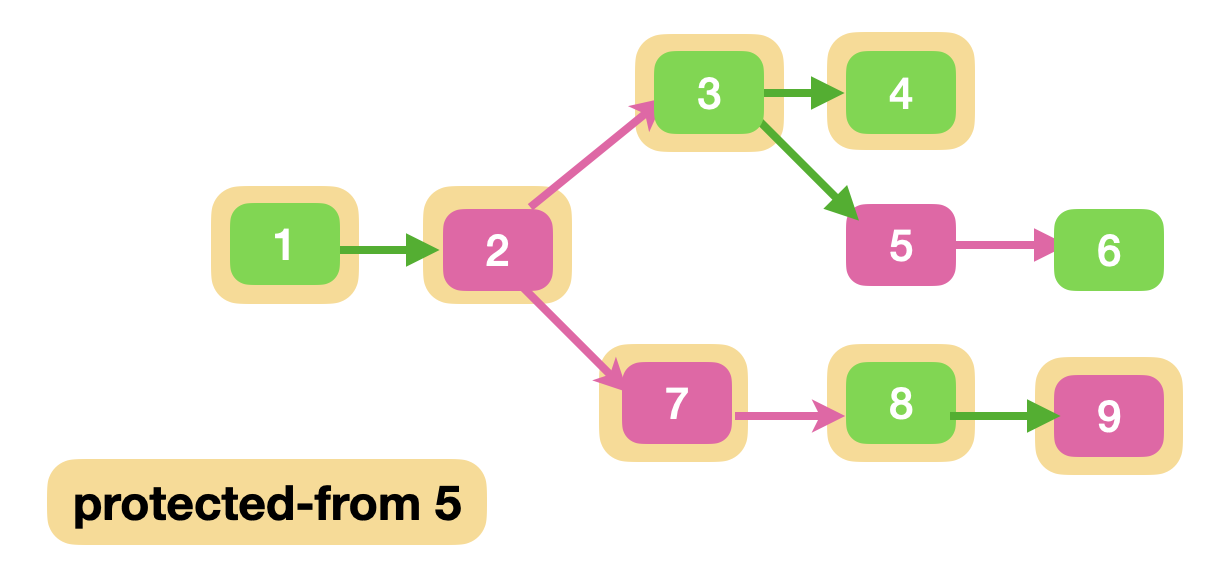
\includegraphics[width=\linewidth]{diagrams/prfA.png}
} 
&
\resizebox{4.5cm}{!}{
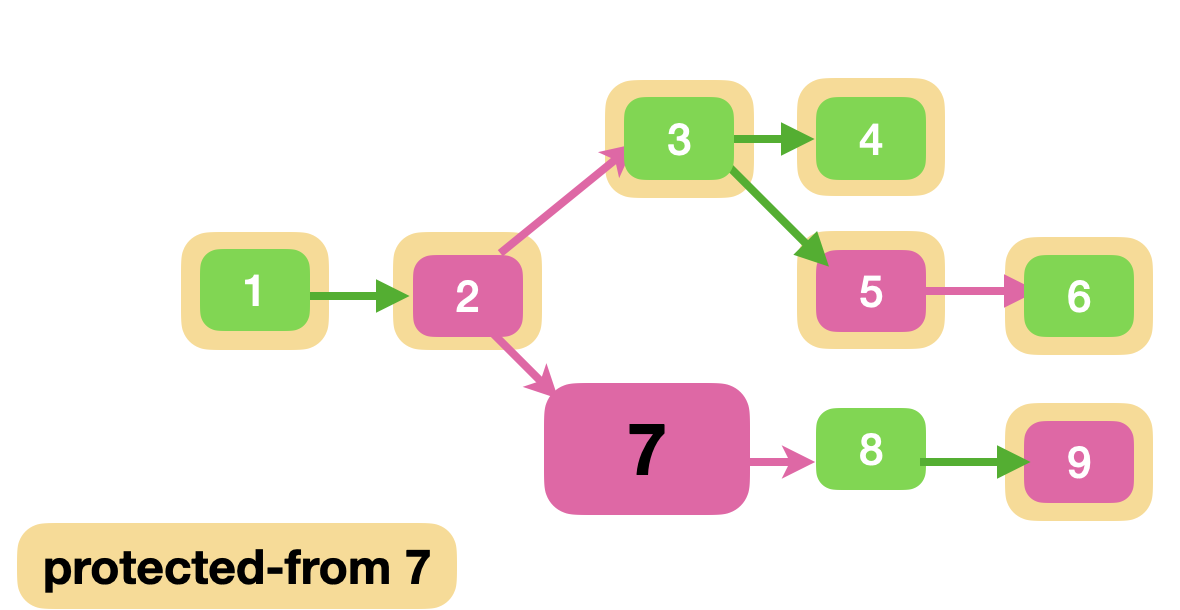
\includegraphics[width=\linewidth]{diagrams/prfB.png}
} 
&
\resizebox{4.5cm}{!}{
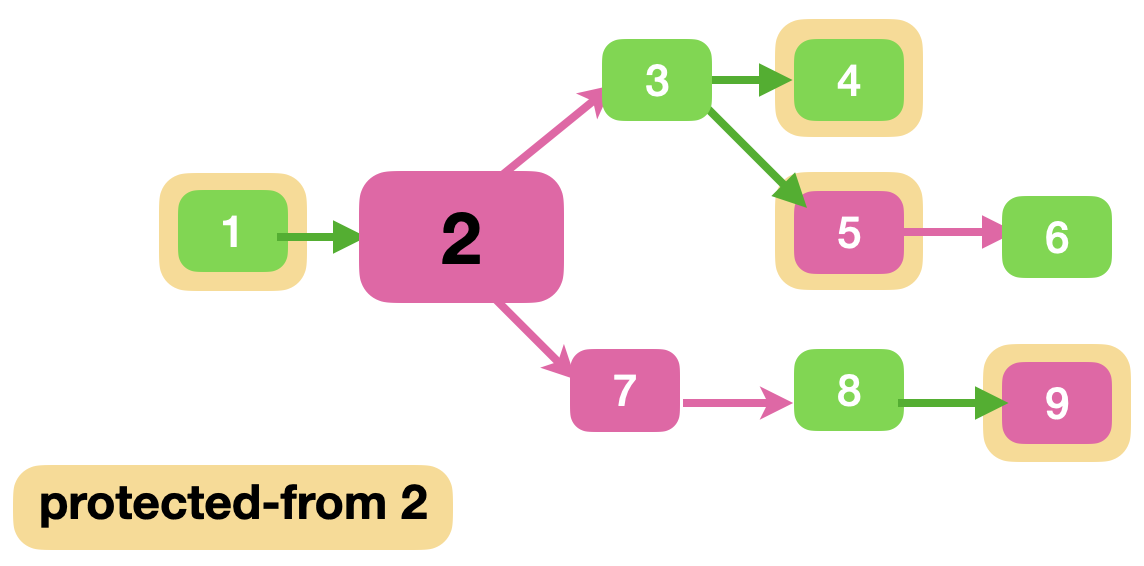
\includegraphics[width=\linewidth]{diagrams/prfC.png}
} 
\\
\hline
protected from $o_5$
&
protected from $o_7$
&
protected from $o_2$
\\
\hline \hline
\end{tabular}
   \caption{Relative Protection. Pink objects are external, and green objects are internal.}
   \label{fig:ProtectedFrom}
 \end{figure}
 
 

%Note that $o_8$ is not protected from $o_2$ because there is a path from $o_2$ to $0_8$ which only traverses external objects. Note also, that even though $o_9$ is external, it is protected from $o_7$.
Note that $o_6$ is not protected from $o_2$. 
Namely, even through there are some internal objects on the path from $o_2$ to $o_6$, in our current model, these objects are not sufficient to prevent eventual, unmitigated access of $o_2$ to $o_6$: it is possible for $o_2$ to make a call to $o_3$, and then this call to return $o_5$. Once $o_2$ has access to $o_5$, it can also get access to $o_6$. 

\vspace{.1in}

We now introduce % the concept of 
(absolute) protection.
An object is protected, if it is protected from all locally reachable {external} objects. This can also be understood as 
``protected from the top frame''. \footnoteSD{TODO: motivate; many external objects, no matter which one has unprotected access to an object }
 
\begin{definition}[Satisfaction 
of Assertions -- Protected] 
\label{def:chainmail-protection}
\label{sect:semantics:assert:prt}
-- continuing definitions from \ref{def:chainmail-semantics} and \ref{def:chainmail-protection-from}:
\begin{enumerate}
\item
$\satisfiesA{M}{\sigma} {\inside {\re}}$  \ \ \ iff \ \ \ 
\begin{enumerate}
\item
{$\forall \alpha.[\ \alpha \in \LRelevantO   {\sigma}\ \wedge\ { \satisfiesA{M}{\sigma}{\external \alpha}} \ \ \Longrightarrow \ \  \satisfiesA{M}{\sigma}{\protectedFrom{\re} {{\alpha}}}\ ] $}, \ \ \ and 
\item
$\satisfiesA{M}{\sigma}{\extThis}\ \ \Longrightarrow\ \ \forall x\!\in\! \sigma.\ \satisfiesA{M}{\sigma}{x\neq \re}$
\end{enumerate}
\end{enumerate}
\end{definition} 
 
% TODO explain
  Figure \ref{fig:Protected} illustrates %the concept of 
  protection. The heap in all three panes is the same as in  Fig \ref{fig:LReachable} and 
 Fig \ref{fig:ProtectedFrom}. State  $\sigma_1$ has  top frame $\phi_1$, which has  one variable, \prg{this}, pointing to $o_1$.  
 State  $\sigma_2$ has  top frame $\phi_2$; it has two  variables,   \prg{this} and \prg{x} pointing to $o_3$ and  $o_7$ resp. 
 State  $\sigma_3$ has  top frame $\phi_3$; it has two  variables,  \prg{this} and \prg{x}, pointing to $o_7$ and $o_3$, resp.  

\begin{figure}[htb]
\begin{tabular}{|c|c|c|}
\hline  
\resizebox{4.5cm}{!}{
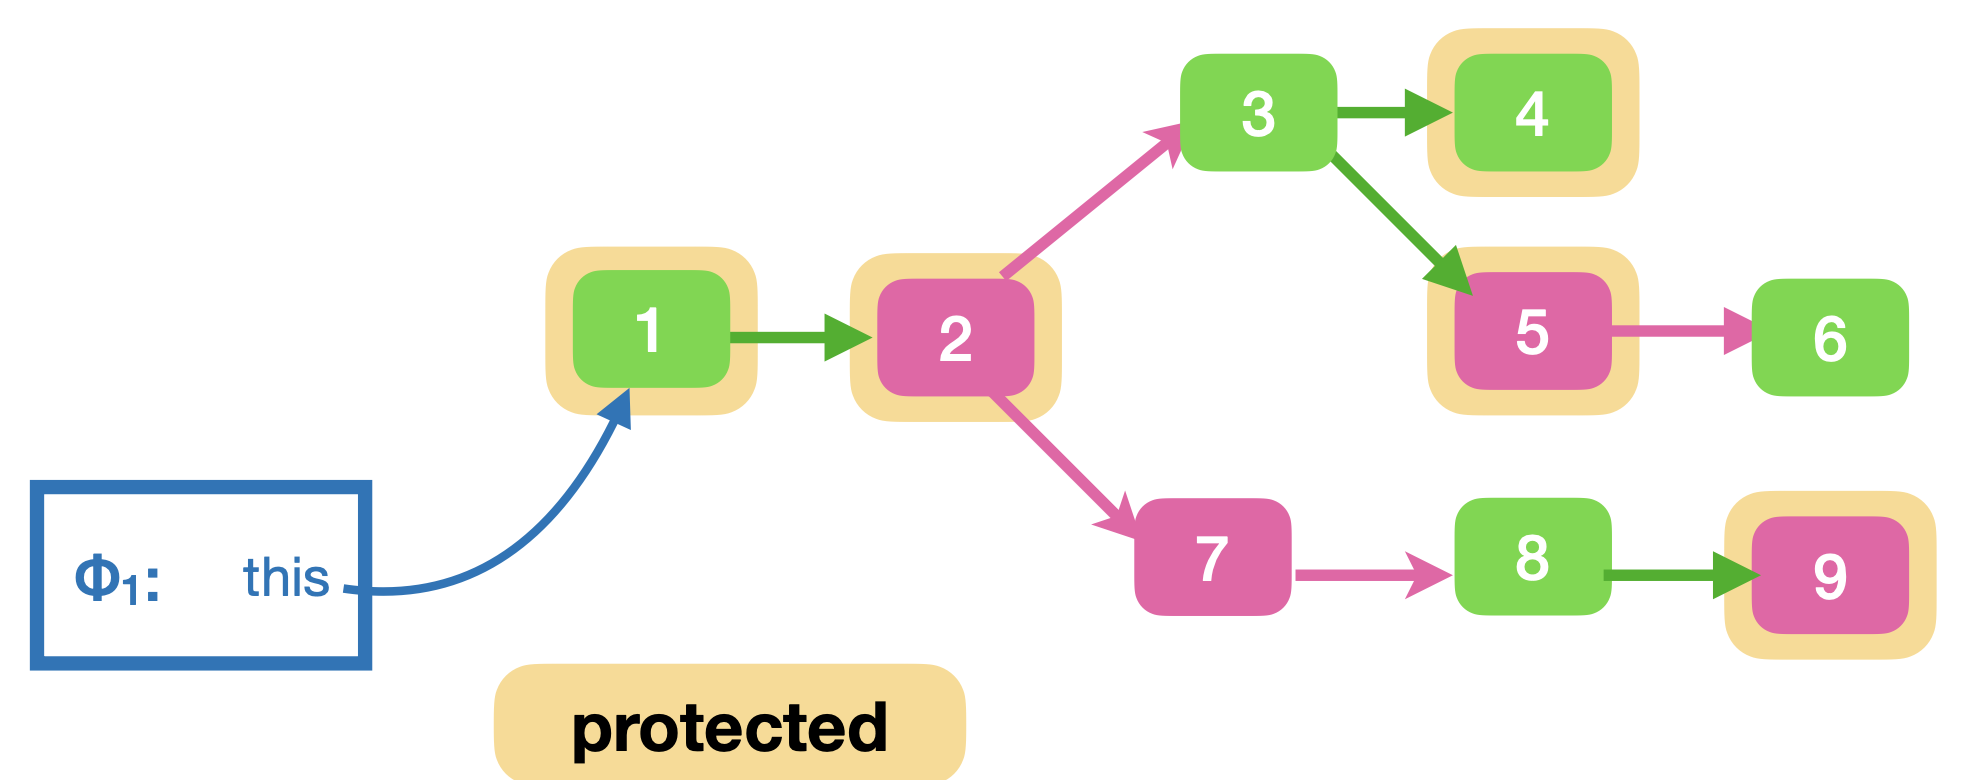
\includegraphics[width=\linewidth]{diagrams/prtFirst.png}
} 
&
\resizebox{4.5cm}{!}{
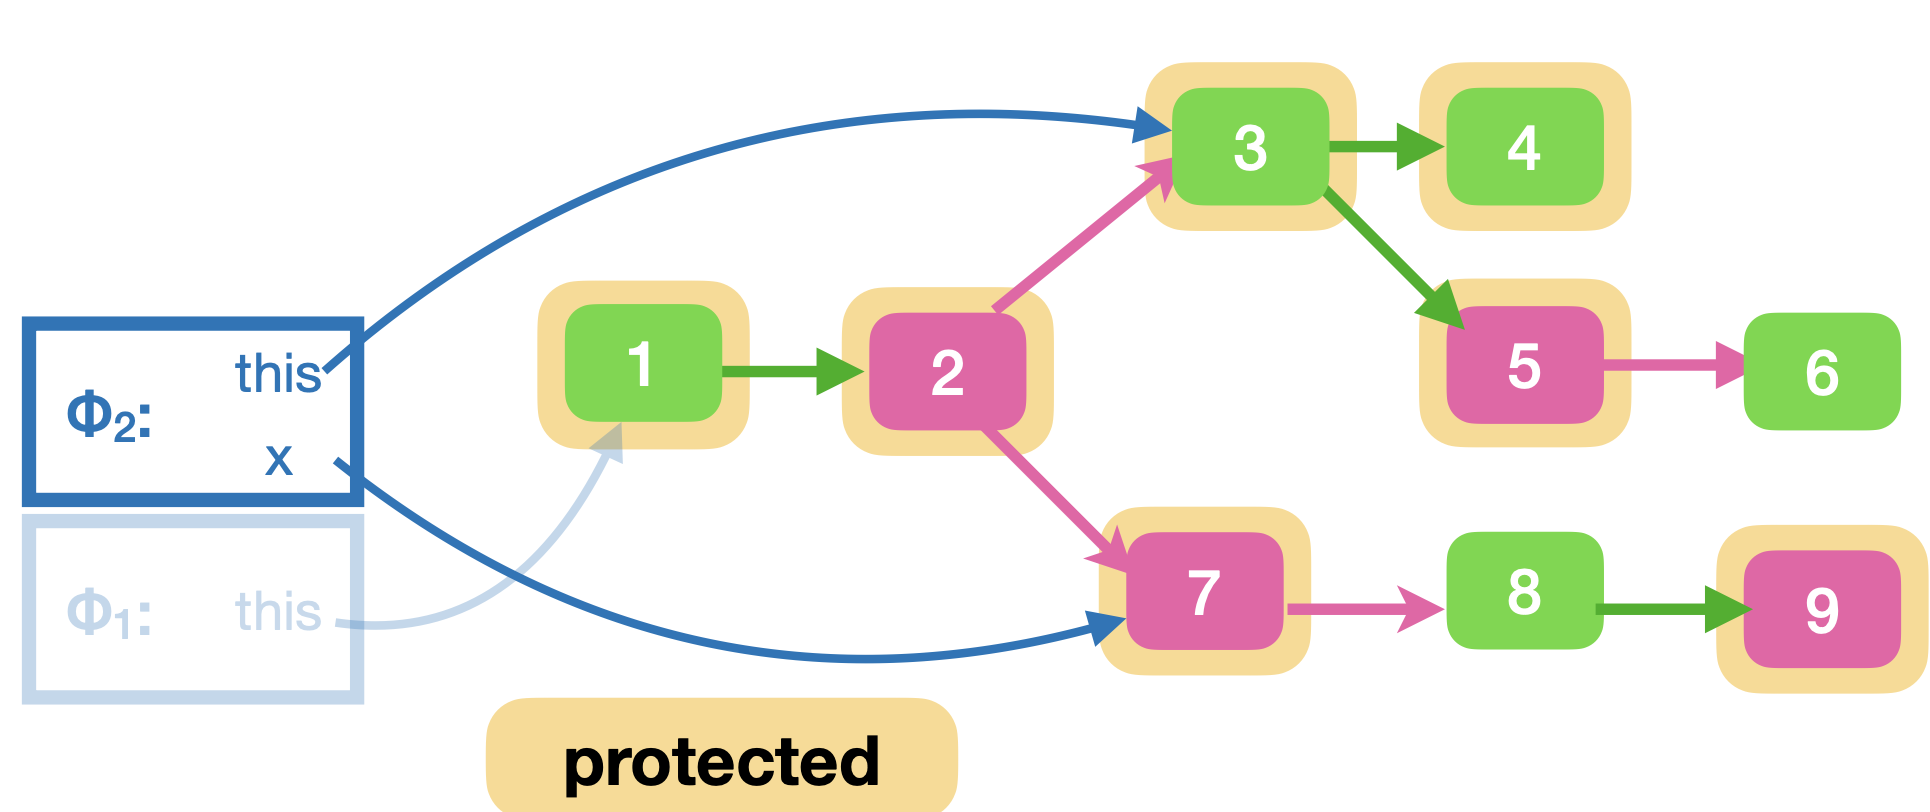
\includegraphics[width=\linewidth]{diagrams/prtSecond.png}
} 
&
\resizebox{4.5cm}{!}{
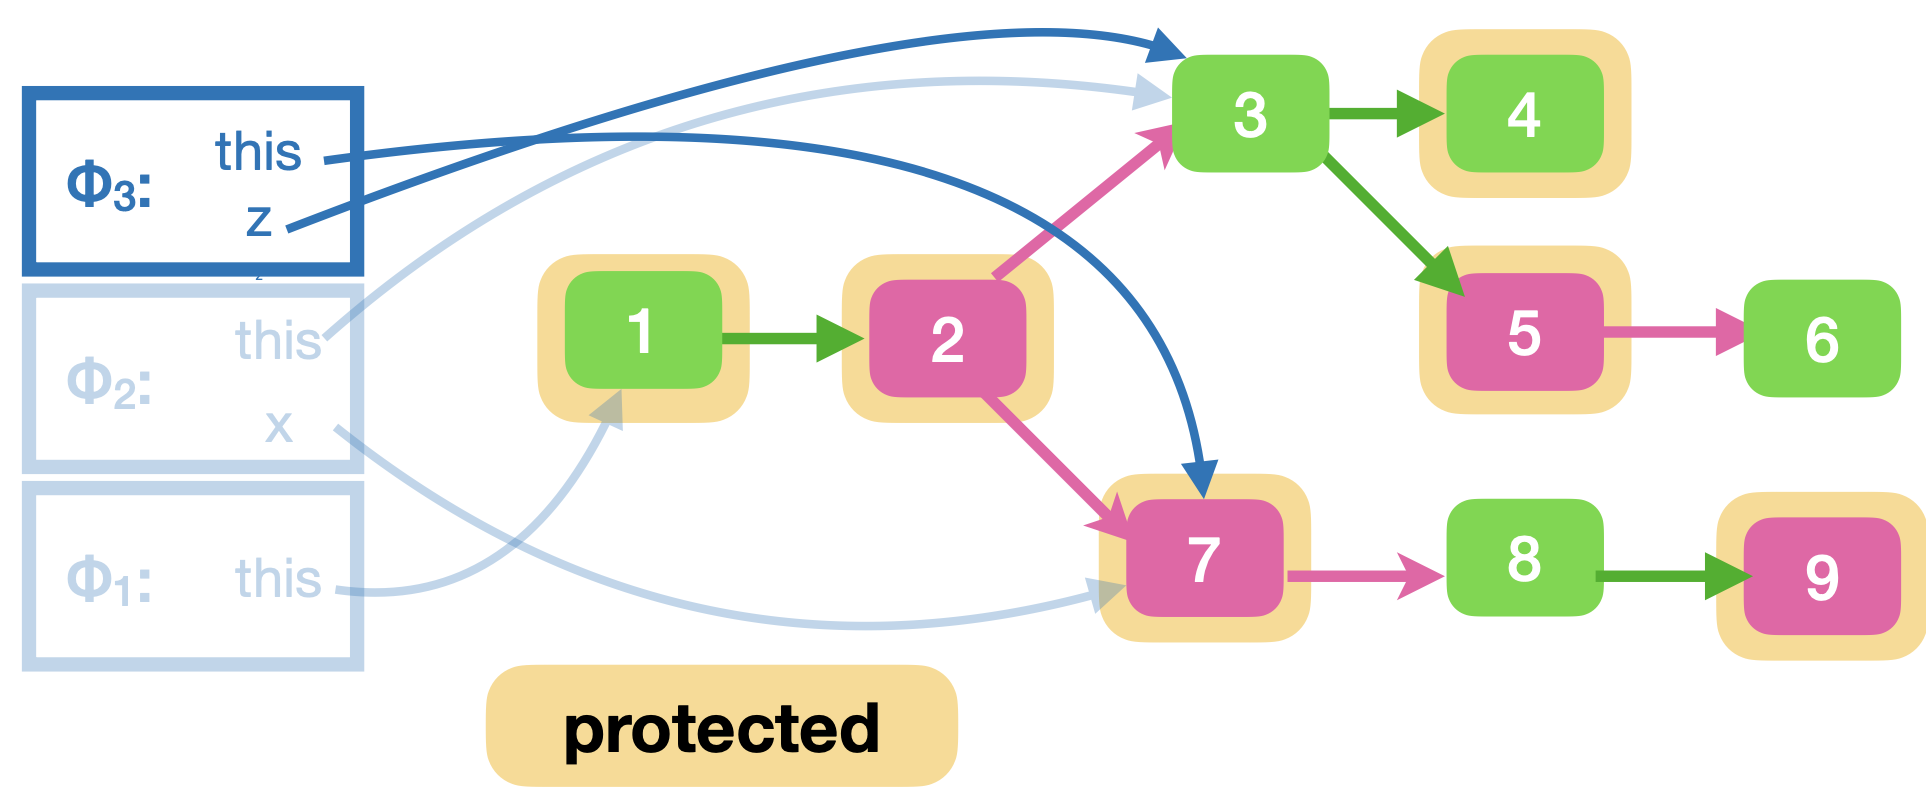
\includegraphics[width=\linewidth]{diagrams/prtLast.png}
} 
\\
\hline
protected in $\sigma_1$ & % with top frame $\phi_1$ &
protected   in $\sigma_2$ & % with top frame $\phi_2$ &
protected  in $\sigma_3$  % with top frame $\phi_2$ &
\\
\hline \hline

\end{tabular}
   \caption{Protected \\
 }
   \label{fig:Protected}
 \end{figure}
 
 
The locally reachable objects in $\sigma_1$ were highlighted in the middle pane of Fig \ref{fig:LReachable}; 
the locally reachable objects from $\sigma_2$  are the same as those from $\sigma_3$, and  were  highlighted in the right pane of that
Fig. 
In Fig.  \ref{gig:Protected} we highlight the protected objects with a golden halo.
 Note that $o_3$ is protected in $\sigma_2$, but is not protected in $\sigma_3$. This is so, because $\interpret {\sigma_3} {\prg{this}}$  is external, and  $o_3$ is an argument to the call. As a result, during the call, $o_7$ may obtain unmitigated access (permission) to $o_3$. 

%\begin{praise}{for protection}
\subsubsection*{Discussion} Protection --- \sdN{objects to which external objects may not get %which objects can get 
unmediated access} % to which other objects 
---  is  a crucial concept: It enables
the verification code in the open world, % even in the presence of
with calls to and callbacks 
from untrusted code.
% ARGHHH a joke citatiion? \cite{praiseYou}.   
Unmediated access is essentially \citet{MillerPhD}'s permission: that we have a ``first
class'' reference to the capability; that we can call any 
method in the capability's public interface; that we can
store or save or present the capability to any other
object to which we've been introduced
%\footnote{``nobody can ever be introduced in a ball-room''}
(compare
2nd-class \cite{rompf-second-class-oopsla2016,rompf-dont-pop-second-class-ecoop2022}
or borrowed (``2nd-hand'') references
\cite{boyland-promises-icse1998,boyland-aliasburying-spe2001}
which are restricted in some way),
without reference to some owning class or defining module.
We discuss alternative designs,
ranging from overly simplistic textual modules \cite{OOPSLA22},
information flow \cite{ddd}, runtime
checks \cite{secure-io-fstar-popl2024},
abstract data type exports \cite{vmsl-pldi2023},
to automated separation-based invariants in
Iris \cite{iris-wasm-pldi2023,cerise-jacm2024},
in section~\ref{sect:related}.
In general, protection is applicable in more situations (i.e.\ is less
restrictive) than most of these approaches,
 \sdN{although more restrictive than the ideal "lack of eventual permission"}. 
\footnoteSD{ HER WHAT IT USED TO SAY:
the contrapositive ideal that lack of eventual permission ensures
lack of effect. Note that ``cannot get unmitigated access'' does not generally imply ``is
protected''. 
}

 
